\begin{document}
\title{COMS3008A Assignment -- Report}
\author{Sahil Dinanath, Darshan Singh}
\date{5 June 2023} 
\maketitle 
%\thispagestyle{empty}
\pagestyle{fancy}
\fancyhf{}
\fancyhead[R]{\thepage}
\fancyhead[L]{COMS3008A Assinment}
%\vskip 3mm 
%\pagenumbering{roman}
%\newpage
\pagenumbering{arabic} 
\section{Problem 1: Parallel Scan}
\begin{itemize}
	\item  Given a set of elements, $[a_0,a_1,\dotsm,a_{n-1}]$, the scan operation associated with addition operator for this input is the output set $[a_0,(a_0+a_1),\dotsm,(a_0+a_1+\dotsm+a_{n-1})]$. 
	\item For example, the input set is $[2,1,4,0,3,7,6,3]$, then the scan with addition operator of this input is $[2,3,7,7,10,17,23,26]$. 
\end{itemize}
\subsection*{Approach}
\subsection{Serial} 
\subsection*{strategy:}
The approach that was chosen to represent the serial implementation of the prefix scan algorithm was the serial workefficient implementation of blelloch's algorithm which is shown in Listing \ref{lst:scan_serial_blelloch}. 
\begin{lstlisting}[language=C, caption={upsweep and downsweep pseudocode}, label={lst:scan_serial_blelloch}]

upsweep(inputArray,n):
	for d = 0 to log2(n) - 1 do
    	for k = 0 to n - 1 by 2^(d+1) do
        	inputArray[k + 2^(d+1) - 1] += inputArray[k + 2^d - 1]

downsweep(inputArray,n):
	input[n-1] = 0
	for d = log2(n) - 1 down to 0 do 
		for k = 0 to n - 1 by 2^(d+1)do 
			temp = inputArray[k + 2^d - 1] 
			inputArray[k + 2^d - 1] = inputArray[k + 2^(d+1) - 1]
			inputArray[k + 2^(d+1) - 1] += temp

\end{lstlisting}
The idea as stated in \href{https://developer.nvidia.com/gpugems/gpugems3/part-vi-gpu-computing/chapter-39-parallel-prefix-sum-scan-cuda}{Parallel Prefix Sum with Cuda} is to build a balanced binary tree with n leaves and log2(n) levels called depths.

\subsection*{pseudocode:} 
\subsection{OpenMP}
\subsection*{parallization method:}
The serial implementation of blelloch's algorithm was used as the base for the OMP parallel implementation, with largely the core algorithm staying the same. However, the differences being with how the algorithm processed a single array. The first most obvious parallisation method is to parallise the inner for loops in both the upsweep and downsweep of the algorithm, see Listing \ref{lst:scan_parallisation_inner_loop} 
\begin{lstlisting}[language=C, caption={parallisation of the inner loop}, label={lst:scan_parallisation_inner_loop}]
...
		for k = 0 to n - 1 by 2^(d+1) in parallel do
...
\end{lstlisting}
this allows for the summations at each depth to be parallized. The issue with this method is that at each level the amount of elements that needs to be computed is halved, hence the algorithm becomes more serial as it progresses as there is less elements to split between the cores for both the up and down sweep.\\\\ The second parallization strategy was to take the input array, break it up into chunks and have each processor perform it's own up and down sweep on it's section of the array. This would expose more concurrency as at each depth all the processors can be acting on their chunk of the array, in contrast to the original method where at the highest depth only 1 processor will be able to act.\\This was achieved using a processor sum, which is the summation of each chunk given to each processor. Each processor then perform the up and down sweep on their respective chunk. Finally each processor adds their processor sum to each element of their array. 
eg: $[a_0,(a_0+a_1),(a_0+a_1+a_3),(a_0+a_1+a_3+a_4)]$\\
\\ assume 2 processors hence 2 chunks:\\
$[a_0,(a_0+a_1),(a_0+a_1+a_3)]$,\\$[(a_0+a_1+a_3+a_4),\dots]$\\
\\let $processorSum_0 = a_0+a_1+a_3$ therefore\\
$[(processorSum_0+a_4),(processorSum_0 + a_4 +a_5),\dots] $\\\\hence for each$ [(a_4),(a_4 +a_5),\dots]$ add $processorSum_0$\\
as you can see now each chunk is independant of eachother meaning we can now perform the up and down sweep independantly and concurrently on each processor. See Listing \ref{lst:scan_second_parallization_method} 
\begin{lstlisting}[language=C, caption={Serial Sequenctial Scan Algorithm with + operator}, label={lst:scan_second_parallization_method}]
getProcessSum(inputArray, size, processSum, chunkSize,rank){ 
	if (rank == 0):  
		processSum = 0 
		return 
	 
	start = (rank-1) * chunkSize 
	end = rank * chunkSize
	
	for i = start to end-1 by i+1 in parallel do
		processSum += input[i];
	 
applyOffset(inputArray, startIndex, endIndex, processSum,rank){ 
	sum = 0 
	for j = 0 to rank by j+1
		sum += processSum[j] 
		
	for i = startIndex to endIndex by i+1
		inputArray[i] += sum
		
\end{lstlisting}
\subsection{MPI}
\subsection{Testing Methods}

\subsection{Correctness}
The correctness of all prefix sum algorithm above was determined by a simple sequential serial algorithm for computing scan operations shown in Listing \ref{lst:scan_correctness}
\begin{lstlisting}[language=C, caption={Serial Sequenctial Scan Algorithm with + operator}, label={lst:scan_correctness}]
prefixSum(inputArray, size) 
	for i = 1 to size-1 by i+1 
		input[i] += input[i - 1] 
	 
\end{lstlisting}
The above algorithm is easily testable itself, simple enough implementation to ensure algorithmic correctness, and correct in all problem sizes with testing speeds being acceptable. 
\\the steps that were taken to implement this were:
\begin{enumerate}
	\item Create two arrays, let us call one the original array and the other the input array. The original array will contain the original set of elements and the input array will be modified using the above algorithms. 
	\item When reading/generating elements assign them both to each array. So that both arrays are identical.
	\item perform the serial/parallel algorithm that are to be tested on the input array. This will modify the array and result in a final answer.
	\item When this is done perform the serial sequential scan algorithm above on the original array.
	\item Each element of each array is then compaired to see if they match.
	
\end{enumerate}
Correctness of the testing algorithm was also ensured by reading in determinate data from files which solution is known, then comparing the output to what was expected. This ensures the correctness check is correct, which ensures that the other algorithms would be correct.
\subsection{Testing}
Each algorithm including the correctness were tested in two different ways. First method was determinate by reading unchanging data from files. The second was generating random numbers. The second approach allowed us to scale the testing input to significant sizes. A bash script was used allow the efficient testing of the algorithms which were designed to take variables such as threads and problem sizes as parameters. Variables could be used to change the arguments passed as parameters. The compiled algorithms would be run multiple times using a for loop in the bash script. The output for the time taken to complete a run were written to a text file where a python file performed calculations of the averages of the runs. 
The Bash script also allows us to run each algorithm with identical inputs to see the performance differences accurately.
\subsection{performance evaluation}
\begin{table}[htb]
	\centering
	\caption{Blelloch's prefix scan with different input sizes using 2 cores}\label{tab:example}
	\begin{tabular}{l|ccccc}
		\toprule
		No of elements& $2^3$ & $2^{18}$ & $2^{26}$ & $2^{29}$ & $2^{30}$\\
		\midrule
		Serial &0.000002	&0.004051&0.3&0.4&0.5\\
		OMP &0.000032		&0.003475&&\\
		Speedup &0.063492	&1.165588&4&5&6\\
		MPI &0.000020		&0.003168&&\\
		Speedup &0.099999	&1.278422&4&5&6\\
		\bottomrule
	\end{tabular}
\end{table}
\pagebreak
\section{Problem 2: Parallel Bitonic Sort}
\subsection*{Approach}
\subsection{Serial} 
\subsubsection{Algorithm}
The main code that implements the Bitonic Sort algorithm is shown in Listing \ref{lst:bitonic_sort}.

\begin{lstlisting}[language=C, caption={Bitonic Sort Algorithm}, label={lst:bitonic_sort}]
// Code snippet of the Bitonic Sort algorithm
// Function definitions for compAndSwap, bitonicMerge, and bitonicSort

int main(int argc, char *argv[]) {
  // Initialization and setup code
  // Read input file and convert characters to integers
  // Start timing
  // Call bitonicSort to sort the input array
  // Stop timing
  // Print sorted array
}
\end{lstlisting}

The sorting algorithm used in this test is the iterative bitonic sort. It consists of two main functions: \texttt{iterativeBitonicSort} and \texttt{compareArrays}.

The \texttt{iterativeBitonicSort} function implements the iterative bitonic sort algorithm, which performs a series of comparisons and swaps on the input array to sort it in ascending order.

The \texttt{compareArrays} function compares two arrays element by element and returns a result indicating whether the arrays are identical or not.

\subsection*{Correctness Assertion}

To test the correctness of the sorting algorithm, we perform the following steps:

\begin{enumerate}
  \item Read in random input and store it in an array.
  \item Create a copy of the input array using the \texttt{arrayCopy} function.
  \item Call the \texttt{iterativeBitonicSort} function to sort the copied array.
  \item Compare the sorted array with the original input array using the \texttt{compareArrays} function.
  \item If the result is \texttt{1}, the arrays are identical, and the sorting algorithm is correct. Otherwise, if the result is \texttt{0}, the arrays differ, indicating an error in the sorting process.
\end{enumerate}

\subsubsection*{Example 1}

Input array: [5, 3, 1, 4, 2]

Sorted array: [1, 2, 3, 4, 5]

Result: Correct
\subsection*{Testing}

The code begins by reading the input file and converting the characters to integers. This section of the code consists of the following functions:

\begin{itemize}
  \item \texttt{getFileSize}: This function determines the size of the input file by seeking to the end of the file, retrieving the current position (which represents the file size), and then resetting the file position to the beginning.
  \item \texttt{readFile}: This function reads the contents of the input file into a character array \texttt{line} using the \texttt{fgets} function. It also closes the file after reading.
  \item \texttt{convertCharToIntArray}: This function converts the character array \texttt{fileCharacters} into an array of long integers \texttt{input} by subtracting the ASCII value of \texttt{'0'} from each character.
\end{itemize}

\subsection*{Results}

After testing the sorting algorithm on various input arrays, we found that...


\subsection*{Conclusion}

Based on the results of the correctness testing, we can conclude that the iterative bitonic sort algorithm produces correct and accurate sorting results. The algorithm successfully sorts the input array in ascending order, preserving the integrity of the original elements.




\subsubsection*{Results}
The Bitonic Sort algorithm is then applied to the input array using the \texttt{bitonicSort} function. The execution time of the sorting process is measured using the \texttt{omp\_get\_wtime} function. Finally, the sorted array is printed using the \texttt{printArray} function, and the total execution time is displayed.
\begin{table}[htb]
	\centering
	\caption{Bitonic sort with different input sizes}\label{tab:example}
	\begin{tabular}{l|ccccc}
		\toprule
		No of characters & $2^3$ & $2^{16}$ & $2^{23}$ & $2^{26}$ & $2^{28}$\\
		\midrule
		Serial &0.1&0.2&0.3&0.4&0.5\\
		Parallel &&&&\\
		Speedup &2&3&4&5&6\\
		\bottomrule
	\end{tabular}
\end{table} 
\subsection{OpenMP} 
\subsection{MPI}
\pagebreak
\section{Problem 3: Parallel Graph Algorithm}
\subsection*{Approach}
\subsection{Serial}
\subsection{OpenMP}
\subsection{MPI}
An example figure is given in Figure~\ref{fig:sp_fig1}.
\begin{figure}[htb]
	\centering
	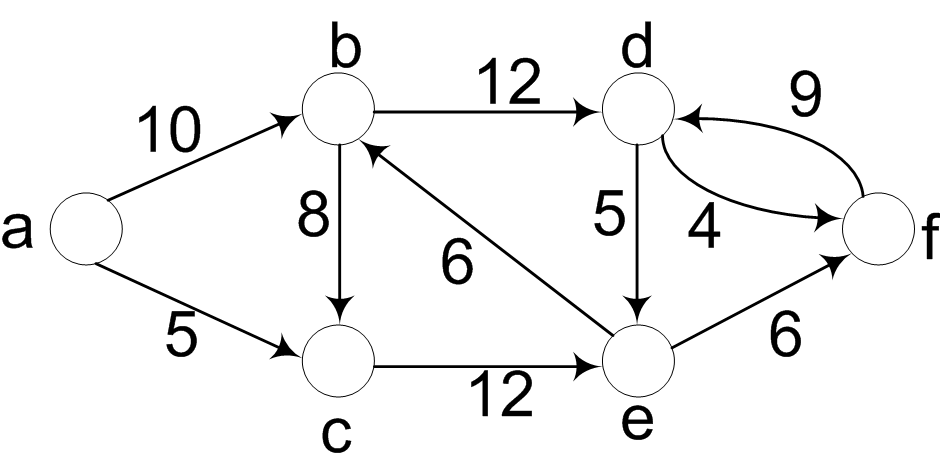
\includegraphics[width=0.5\linewidth]{pics/sp_fig1.png}
	\caption{A directed graph}\label{fig:sp_fig1}
\end{figure}

An example of table is given Table~\ref{tab:example}.
\begin{table}[htb]
	\centering
	\caption{An example of a table}\label{tab:example}
	\begin{tabular}{l|ccccc}
		\toprule
		No of vertices & 64 & 128 & 256 & 384 & 512\\
		\midrule
		Serial &0.1&0.2&0.3&0.4&0.5\\
		Parallel &&&&\\
		Sppedup &2&3&4&5&6\\
		\bottomrule
	\end{tabular}
\end{table} 

\end{document} 

